\section{Linux Audit Framework}
\label{sec:audit}



  The Linux Audit system \cite{suse2004} provides a way to observe and analyse system activities. 
  While Linux Audit can be configured to monitor high-level activities such as login attempts \cite{audit}, its primary utility (and overhead) comes from tracking low-level system calls, which is the focus of this paper.
  An overview of the Linux Audit architecture is presented in Figure \ref{fig:audit_arch}. 
  When an application invokes a system call (\textcircled{1}),
    the subsequent kernel control flow eventually traverses an {\tt audit\_filter} hook (\textcircled{2}).
    \begin{figure}[t!] 
        \centering
        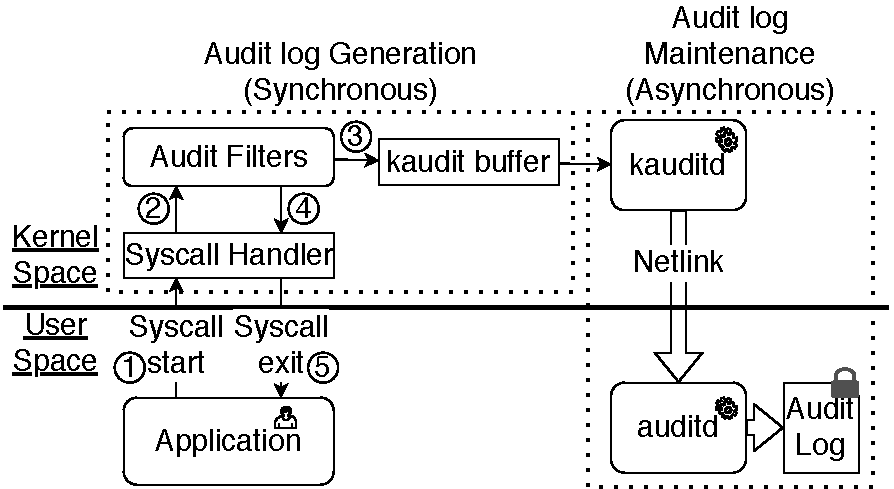
\includegraphics[width=\linewidth]{fig/audit_arch_2.pdf}  
        \caption{\label{fig:audit_arch} Architecture of Linux Audit Framework. Audit logs are generated using auditing hooks in kernel's system call (Syscall) handler and temporarily stored in the kaudit buffer. Log maintenance is handled by two background daemons, kauditd and auditd.}
      \end{figure} 
  Linux Audit examines the context of the event and compares it to pre-configured audit rules,
    generates a new log event and enqueues it in a message buffer if there is a match (\textcircled{3})
    before returning control to the system call handler (\textcircled{4}) and then to the application (\textcircled{5}).
  Asynchronous from this workflow, a pair of (non-real-time) audit daemons, {\tt kauditd} and {\tt auditd}, that run in kernel and user spaces respectively,
    empty the message buffer to user space for storage, distribution and analysis.
  Because the transport of logs is asynchronous, it is possible for the kaudit buffer to overflow if
    system calls occur faster than the daemon flushes to user space,
    creating the potential for event loss.  